%\subsection{Experiments and results}
\subsection{Settings}

\textbf{Data.} We randomly split all words in WIST into three parts, 2,500/5,000 as development/test data and remaining as training data. 
%We conduct experiments on our manually annotated char-level syntactic treebank, which consists of 25,531, 2,504, and 5,013 words in training, development, and test sets respectively.

\textbf{Hyperparameters.} 
We set the dimension of char embeddings to 100. 
We obtain pre-trained character embeddings by training  word2vec on Chinese Gigaword Third Edition.
%We adopt the 100 dimension character embeddings of %\citet{liying-2019} 
%pretrained with word2vec model on Chinese Gigaword.
In order to see effect of contextualized character representations, we apply BERT \cite{devlin-2019-bert} \footnote{BERT-base-Chinese:\url{https://github.com/google-research/bert}} to each word as a char sequence. The output vectors of the top four layers are concatenated and reduced into a dimension of 100 via an MLP. 
For other hyper-parameters, we keep the default configuration in SuPar.
%We adopt most of the parameter settings in the open source parser \cite{dozat2016deep}. 
%Each model is trained for at most 1000 iterations. We stop training when the peak performance on the development data does not increase in 100 consecutive iterations. 


%The dimension of char embedding is set to 50. 
\textbf{Evaluation metrics.} 
We adopt the standard unlabeled and labeled attachment score (UAS/LAS), i.e., the percent of characters that receives the correct head (and label). 
%The unlabeled and labeled complete matches (UCM/LCM) is the percent of words having correct whole trees.
The complete match (CM) is the percent of words having correct whole trees.

\setlength{\tabcolsep}{3.6pt}
\begin{table}[tb]
%\setlength{\leftskip}{-25pt}
\begin{center}
% \begin{small}
\begin{tabular}{l  rr rrr }
\toprule
\multirow{2}{*}{} 
& \multicolumn{2}{c}{Dev }
& \multicolumn{3}{c}{Test} \\
\cmidrule(lr){2-3} \cmidrule(lr){4-6}
% \cline{2-6}
& UAS & LAS & UAS & LAS & CM\\
\hline
Random & 81.18 & 76.15  & 80.63 & 75.58 & 65.13 \\[2pt]
%\hline
\multirow{2}*{Pretrained}
 & 82.42 & 77.30 & 81.64 & 76.98  & 67.09 \\
 & +1.24 & +1.15 & +1.01 & +1.40 & +1.96\\[2pt]
%\hline
\multirow{2}*{BERT} 
 & 88.27 & 85.18 & 88.33 & 84.98 &77.72\\
 & +5.85 & +7.88 & +6.69 & +8.00 & +10.63\\
\bottomrule
\end{tabular}
% \end{small}
\caption{Results of word-internal structure parsing using different character representations.} 
\label{iwdp-result}
\end{center}
\end{table}


\subsection{Results}

Table \ref{iwdp-result} shows the main results  %word-internal structure parsing 
under different char representations.  
% It turns out that word-internal structure parsing is not a piece of cake.
% The best model integrated BERT representations\footnote{The BERT in the experiment is ``bert-base-chinese'' released by \citet{peters2018deep}.}, which outperforms those without BERT  by over 10 in LAS, merely achieves a LAS of 84.98 and a LCM of 77.72.
% Pretrained char embeddings are also helpful to the word-internal structure parsing.
% But it only brings improvement by 1.40 in LAS and 1.96 in LCM, compared with the model using randomly initialized char embeddings.
It is obvious that using randomly initialized char embeddings, the parser can only reach about 76 in LAS. This shows that parsing word-internal structure is very challenging without using extra resources. 
When we pretrain char embeddings on large-scale labeled data, the performance can be consistently improved by over 1 point in both UAS/LAS, and nearly 2 points in CM. 
Finally, employing the contextualized character representations dramatically improves performance further by about 6/8/10 points in UAS/LAS/CM. 

However, even with BERT, model performance still lags behind averaged human performance (90.9 in LAS) by large margin.
Our experienced annotators can even reach more than 94. 
Our experience in manual annotation points out two possible directions to enhance the model: 1) making use of sentence-level contextual information; 2) leveraging the meanings in dictionaries, usually in the form of explanation or example sentences. 
We leave them for future exploration. 

%without  using pretrained char embeddings brings substantial improvement by 1.40 in LAS and 1.96 in LCM on test. 

%Integrating with BERT representations\footnote{The BERT in the experiment is ``bert-base-chinese'' released by \citet{peters2018deep}.} can further boost the model performance by a very large margin, outperforming those without BERT by over 8 in LAS and over 10 in LCM on test. 

\textbf{Analysis on label-wise accuracy.}
% Using BERT representations can further improve the parser by a very large margin.
%\begin{figure}[tb]
  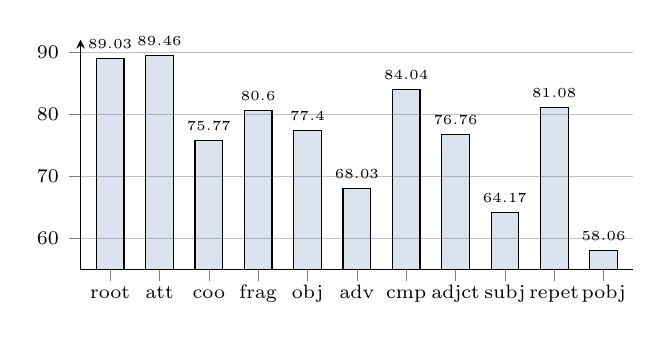
\begin{tikzpicture}
    \begin{axis} [
        width=8.6cm, height=4.5cm,
        ybar,
        axis y line=left,
        axis x line=left,
        x axis line style={-},
        ymajorgrids=true,
        enlarge x limits=0.06,
        tick align=outside,
        ymin=55, ymax=92,
        symbolic x coords={
            root, att, coo, frag, obj, adv, cmp, adjct, subj, repet, pobj
        },
        xtick=data,
        nodes near coords=\pgfmathprintnumber\pgfplotspointmeta,
        xticklabel shift=6,
        x tick label style={anchor=base, font=\scriptsize},
        y tick label style={font=\scriptsize},
    ]
    \addplot [
        draw=black,
        fill opacity=0.2, 
        text opacity=1,
        font=\tiny, 
        fill={rgb,255:red,76; green,114; blue,176}] coordinates {
        (root, 89.03)
        (att, 89.46)
        (coo, 75.77)
        (frag, 80.6)
        (obj, 77.4)
        (adv, 68.03)
        (cmp, 84.04)
        (adjct, 76.76)
        (subj, 64.17)
        (repet, 81.08)
        (pobj, 58.06)
    };
  \end{axis}
\end{tikzpicture}

\caption{
  Accuracy on different dependency labels.
}
\label{fig:model-acc}
\end{figure}

The second major row in Table \ref{table:label distribution} reports accuracy regarding different labels for the model with BERT. 
The model achieves the highest accuracy on ``att'' and ``root'', possibly because the two labels take very large proportion in the data for sufficient model training. 
%One direct reason is that these two labels accounts for the largest proportion of all labels, and thus the model can be trained sufficiently. 
% , indicating that it is relatively easy for the model to recognize the head character for each word.
%Moreover, it is easy to recognize ``att'' since the word with ``att'' label usually has a typical modifier-noun structure, which is very common in Chinese words and usually frequently occurs in the training data. 
%For ``root'', it represents the most important head character that conveys the main meaning of each word, such head characters are also high-frequency characters and thus can be distinguished with other unimportant characters. 
By contrast, ``pobj'' and ``subj'' have the lowest accuracy, and are difficult for models as well as discussed in Section \ref{sec:data-annotation}. 
%performance, achieving only ``58.1'' in accuracy.
%By carefully checking the predicted results, we find that the model usually confuses ``pobj'' with ``obj''. In fact, these two labels are quite similar in syntax. The proportion of ``obj'' is much larger than ``pobj'' (5.4 vs. 0.2). The sample imbalance problem causes the model to lean to label ``pobj'' as ``obj''.
This leads to 
another observation that model accuracy is roughly correlated with annotation accuracy, implying the difficulties for human and model are usually consistent. 
% However, it is not easy for the model to correctly recognize ``subj'' and ``pobj'', achieving only ``64.2'' and ``58.1'' in accuracy respectively. By carefully checking the predicted results, we find that the model usually confuses ``subj'' with  ``adv'' and confuses ``obj'' with ``pobj''.

% the sample imbalance problem causes the model to lean to label “激动(excite)” as an adjective



% as illustrated in Table \ref{table:label distribution}, and thus the model can be trained sufficiently. 

% coo和adv容易混淆

% and ``att''

% the proportion of these 

% account for a relatively large proportion in all the labels


% whereas the lowest accuracy on ``subj'' and ``pobj'', which is consistent with the manual annotation accuracy.



% root和att准确率高是因为:1.root标签属于核心字,是一个词中最为核心的部分,往往承载着一个词的主要意思,因此比较容易找出。att标签准确率高我觉得是因为att标签数量多,如果核心字是名词性字,那么它前面的字很有可能是att,容易识别,特征明显。subj难识别是因为,subj标签容易被误标注成adv标签,对于是主语还是修饰关系,有时候难以理解,pobj标签错误率高更大原因是因为难以分辨到底是obj还是pobj,比如在这个字,一般认知下会觉得是介词,但是其实在单个字中,在通常作为动词,形成obj


